% Asset ID: AS2CorrelationAndRegressionLinesTikZ-002
% Source: CCEA AS2-DPI-LO004 + S1-Chp4-Correlation.pdf page 5
% Related section: Key Definitions and Notation
% Purpose: Label independent/explanatory and dependent/response variables.
\documentclass[tikz,border=6pt]{standalone}
\usepackage{amsmath}
\usetikzlibrary{arrows.meta,positioning}
\begin{document}
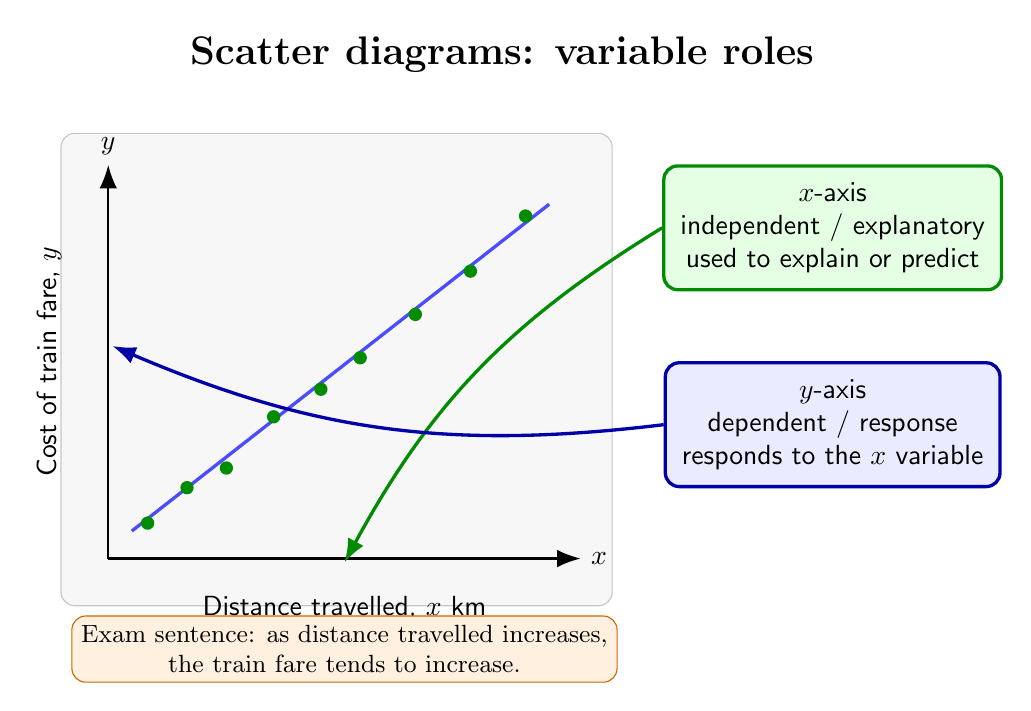
\begin{tikzpicture}[font=\sffamily,>={Latex[length=3mm]},point/.style={circle, fill=green!55!black, inner sep=1.7pt},card/.style={draw, rounded corners=5pt, very thick, align=center, inner sep=6pt}]
\node[font=\bfseries\Large] at (5,6.4) {Scatter diagrams: variable roles};
\draw[rounded corners=5pt, fill=gray!6, draw=gray!45] (-0.6,-0.6) rectangle (6.4,5.4);
\draw[->, thick] (0,0) -- (6,0) node[right] {$x$};\draw[->, thick] (0,0) -- (0,5) node[above] {$y$};
\draw[very thick, blue!70] (0.3,0.35) -- (5.6,4.5);
\foreach \p in {(0.5,0.45),(1.0,0.9),(1.5,1.15),(2.1,1.8),(2.7,2.15),(3.2,2.55),(3.9,3.1),(4.6,3.65),(5.3,4.35)}\node[point] at \p {};
\node[below] at (3,-0.35) {Distance travelled, $x$ km};\node[rotate=90] at (-0.75,2.5) {Cost of train fare, $y$};
\node[card, fill=green!10, draw=green!55!black] (xcard) at (9.2,4.2) {$x$-axis\\independent / explanatory\\used to explain or predict};
\node[card, fill=blue!8, draw=blue!65!black] (ycard) at (9.2,1.7) {$y$-axis\\dependent / response\\responds to the $x$ variable};
\draw[->, very thick, green!55!black] (xcard.west) to[bend right=15] (3,-0.05);\draw[->, very thick, blue!65!black] (ycard.west) to[bend left=15] (0.05,2.7);
\node[draw=orange!80!black, fill=orange!12, rounded corners=5pt, align=center, font=\small] at (3,-1.15) {Exam sentence: as distance travelled increases,\\the train fare tends to increase.};
\end{tikzpicture}\end{document}
